\documentclass[14pt,a4paper]{article}
\usepackage[utf8]{inputenc}
\usepackage[T1]{fontenc}
\usepackage{amsmath}
\usepackage{amsfonts}
\usepackage{amssymb}
\usepackage{graphicx}
\usepackage{hyperref}
\usepackage[style=authoryear,backend=biber]{biblatex}
\DeclareDelimFormat{postnotedelim}{\addcomma\space}
\usepackage{csquotes}
\usepackage[margin=3.5cm]{geometry}
\usepackage{titlesec}
\usepackage{appendix}
\usepackage{booktabs}
\usepackage{longtable}
\usepackage{fancyhdr}
\usepackage{xurl}

\addbibresource{references.bib}

\titleformat{\section}
  {\normalfont\Large\bfseries}{\thesection}{1em}{}
\titleformat{\subsection}
  {\normalfont\large\bfseries}{\thesubsection}{1em}{}

\title{Strategic BPMN 2.0 Modelling}
\author{Process-Centric Analysis of the Car Repair Shop Case Study}
\date{}

\renewcommand{\labelitemi}{-}

\pagestyle{fancy}
\fancyhf{}
\renewcommand{\headrulewidth}{0.4pt}
\renewcommand{\footrulewidth}{0.4pt}
\fancyhead[L]{UFCFAF-30-3 | Development of Information Systems Projects}
\fancyhead[R]{Page \thepage}
\fancyfoot[C]{\thepage}

\begin{document}

\maketitle

\hrule

\vspace{3em}

Word Count: 927

\vspace{3em}
\hrule

\vspace{2em}
\textbf{Abstract}
\vspace{1em}

This paper presents a strategic business process model for the Car Repair Shop case study, translating socio-technical i* requirements into a coherent Business Process Model Notation (BPMN) representation. By observing the transformation of actor dependencies and intentional elements into process flows, the essay addresses the strategic model's capacity to bridge gaps between stakeholder goals and rapidly achievable operational function. Focus on critical process touchpoints, participant interactions, and decision gateways, allows developers to prioritise comprehensibility over comprehensive detail to best serve development as a visual guide to the mapping of real world to virtual abstraction. The resulting BPMN model provides a foundation for executive oversight and subsequent operational elaboration, communicating business logic effectively whilst preserving essential socio-technical elements captured in goal-oriented requirements engineering.

\vspace{3em}
\hrule

\thispagestyle{empty}

\tableofcontents
\pagenumbering{roman}

\newpage

\pagenumbering{arabic}

\section{Introduction}

Strategic business process models serve as essential intermediaries between high-level socio-technical models and operational implementations, providing what \textcite[p. 76]{Silver2011} describes as the "crucial abstraction layer" that frames enterprise processes and builds upon our previously established i* socio-technical model.

These models serve distinct purposes from their operational counterparts, enabling executive comprehension through the omission of superfluous and superficial details. As \textcite[p. 152]{Dijkman2011} note, "strategic models prioritise communication efficacy over execution specificity," making them valuable tools for managerial organisation. For a Car Repair Shop, where complex dependencies exist between customers, reception staff, mechanics, and towing services, a strategic BPMN model visualises essential service flows whilst abstracting or simplifying complexities away.


\begin{figure}[ht]
  \hspace{-6.5em}
    \begin{minipage}[t]{1.3\textwidth}
        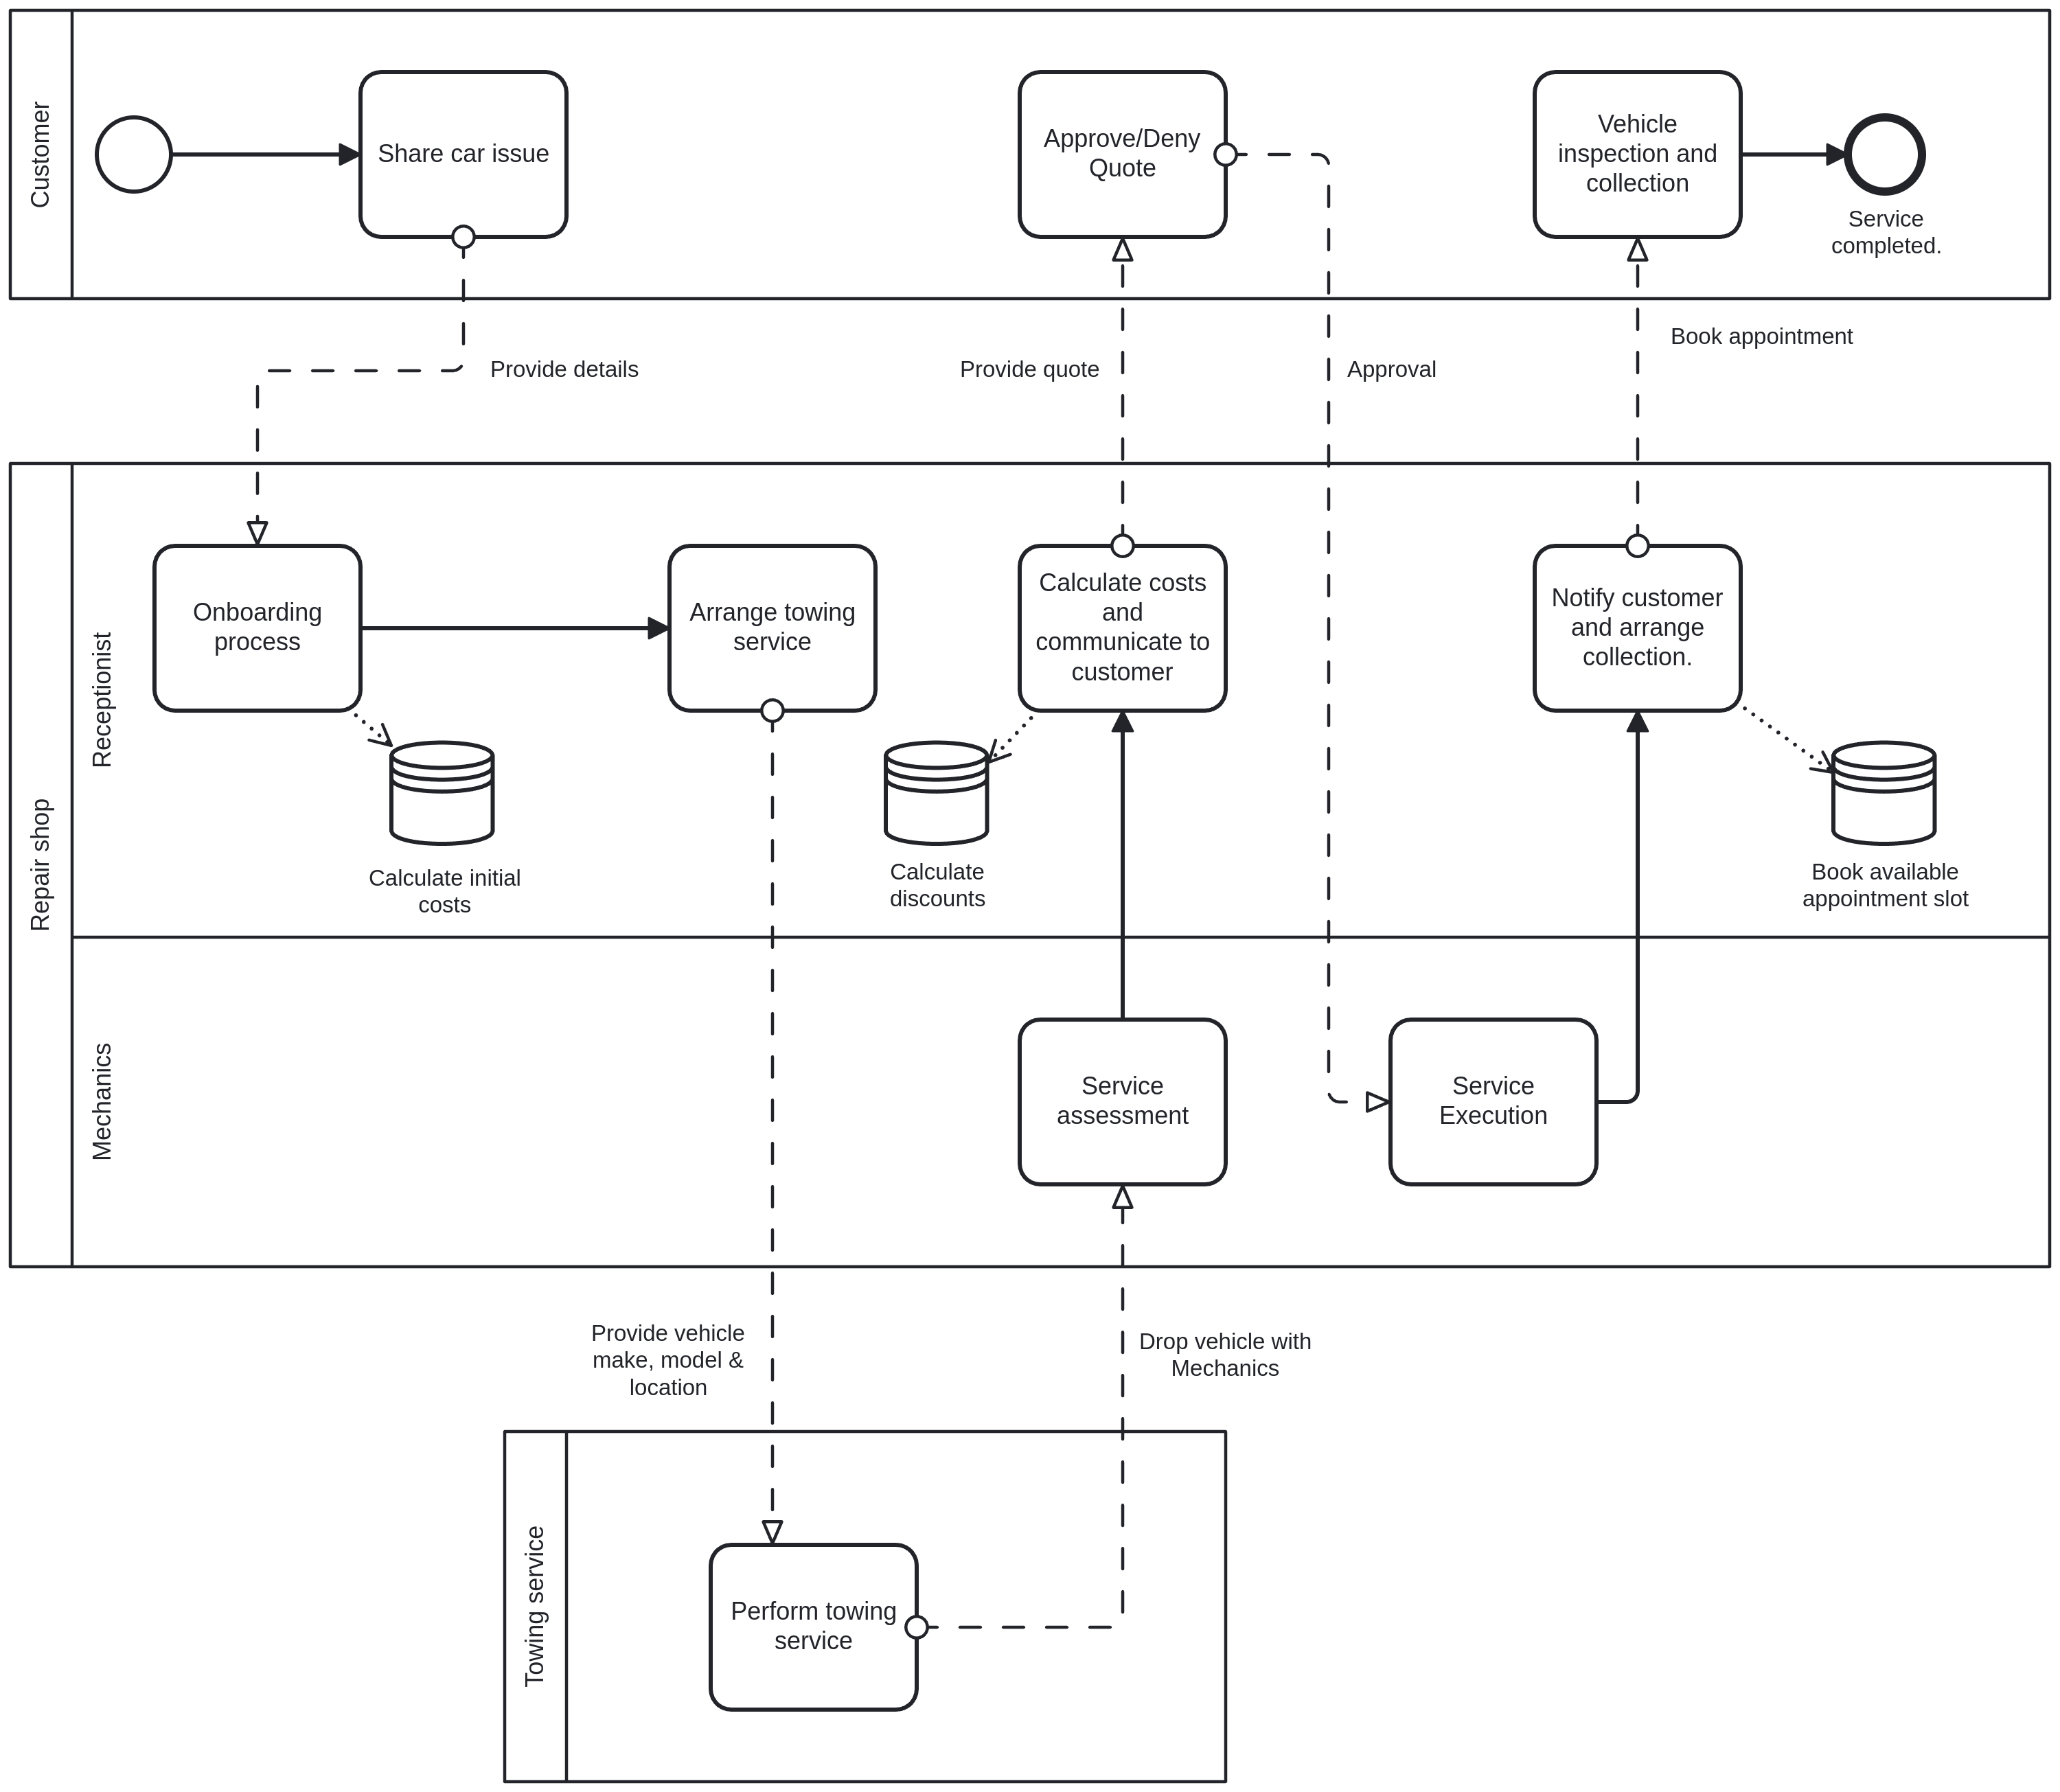
\includegraphics[width=\linewidth]{strategic.png}
        \caption{BPMN 2.0, Strategic Business Process Model}
    \end{minipage}
\end{figure}

\section{Theoretical Foundations and Methodology}

Strategic modelling using BPMN serves a distinct and necessary use case in the business process hierarchy. According to \textcite[p. 17]{Allweyer2016}, strategic models "provide the high-level process architecture within which operational concerns exist," focussing on what \textcite[p. 89]{Dumas2018} term "core process patterns rather than execution variations." The translation from goal-oriented requirements to process models represents a methodical and measured initial shift from intentional modelling to process flow. As \textcite[p. 342]{Dalpiaz2016} observe, this transformation "converts actor dependencies and rationales into sequential activities with defined handoffs."

\vspace{0.7em}
Our methodology, comprised three distinct phases:

\begin{itemize}
  \item Actor mapping to pools and lanes.
  \item Dependency \& relationship constraint conversion to message flows.
  \item Task and goal transformation into activities and events.
\end{itemize}

This approach preserved socio-technical elements whilst maintaining comprehensibility, limiting diagram complexity, and focussing on the "happy path" process flow. As alluded to by \textcite[p. 136]{Corradini2018}'s quality criteria framework - syntactic correctness, semantic adequacy, and pragmatic effectiveness were key characterics to validate in the finished product.

\section{Pool Structure and Participant Boundaries}

Our strategic BPMN model establishes clear boundaries between four primary participants, discrete from each other in their own pool: Customer, Receptionist, Mechanic, and Towing Service. Delineating these boundaries as "primary organisational units or external stakeholders" \textcite[p. 103]{Kluza2017} as opposed to mere functional subdivisions exposes requirement for certain communications to cross organisational boundaries. This in turn can help to pinpoint key integration points warranting particular attention in the system's development.

The Receptionist pool serves as a nexus and merits particular consideration due to its essential function as coordinator of the system. Unlike the Mechanic pool, which contains technically specialised activities, the Receptionist manages interactions, not independently but with all other participants, illustrating why this role functions as what \textcite[p. 48]{Gorton2017} identify as the "primary integration point" between customer requirements and technical execution.

\section{Strategic Activities and Process Phases}

The model captures four essential process phases - each containing significant activities that elucidate those certain process elements warranting executive attention:

\begin{enumerate}
    \item \textbf{Initiation Phase} – The customer's "Share car issue" activity and the receptionist's "Onboarding process" establish the service relationship. The conditional activation of towing services demonstrate flexibility at this stage - reflecting the reality that the customer's need from the very first interaction has a high degree of variance.

    \item \textbf{Assessment Phase} – The mechanics' "Service assessment" activity drives the diagnostic process that informs the receptionist's "Calculate costs and communicate to customer" activity. The separation ensures technical expertise informs customer commitment - emphasising the relationship between diagnosis and quotation.

    \item \textbf{Approval and Execution Phase} – The customer approval/denial gateway is a prime example of customer agency fundamentally shaping process flow. This decision point represents what \textcite[p. 185]{Allweyer2016} term a "business-critical divergence point" where customer choice determines whether value-generating activities proceed.

    \item \textbf{Completion Phase} – The notification and collection activities culminate in demonstrate conclusion of the process - explaining the coordination requirements between mechanics, receptionist, and customer. The ultimate aim of the entire system process is to complete successfully.
\end{enumerate}

These activities directly correspond to critical dependency relationships identified in the i* framework, including membership programme integration that \textcite[p. 263]{Castro2018} characterised as a "strategic feedback loop."

\section{Communication Patterns and Message Flows}

Key message flows and the mapping of information exchange reveal the most critically influential communication dynamics for process success:

\begin{enumerate}
    \item \textbf{Customer-Receptionist Communication} – Three critical information exchanges (service request, quote provision and approval, pick-up coordination) that define the customer experience lifecycle.

    \item \textbf{Receptionist-Mechanics Workflow} – Service request and completion notifications that coordinate the core repair process, reflecting the resource dependencies identified in the socio-technical model.

    \item \textbf{Triangular Communication Pattern} – The interaction between Customer, Receptionist, and Towing Service creates what \textcite{Corradini2018} characterise as a "coordination-intensive subprocess" requiring careful information system support.
\end{enumerate}

The resulting communication patterns reveal why certain process configurations create coordination challenges that warrant executive attention. These message flows represent what \textcite[p. 195]{Delgado2020} term "critical handoff points requiring careful integration" in subsequent operational models and system implementation.

\section{Conclusion}

The translation from i* socio-technical models to a strategic BPMN representation provides essential architectural framing for a high-level overview of the business logic from start to finish. This strategic model maintains focus on critical business dynamics while abstracting operational complexities, creating what \textcite[p. 103]{Bosch2018} describe as "the essential communication bridge between executive foresight and operational execution."

As a foundation for a subsequent elaboration, and the next stage of BPMN, the strategic model establishes process boundaries, identifies integration requirements, and quantifies business measures and opportunities - all whilst maintaining concise and simple flows for full reader comprehension. Through this deliberate abstraction, the BPMN model fulfils its essential purpose as a strategic communication tool that frames implementation decisions within the broader organisational context of the Car Repair Shop.

\newpage

\printbibliography

\end{document}
